\section{Fiche du Pérou}

Date: 10/10/2009

\begin{multicols}{2}

\textbf{\textsc{Drapeau}}

\hspace*{-0.65cm}
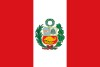
\includegraphics[width=4.8cm]{articles/Fiche-du-perou/1255177646Fug0.jpg}
Drapeau du Pérou

\textbf{\textsc{Le Pérou en chiffres}}

** Capitale : ** Lima
** Superficie ** : 1.285.216km2
** Habitants ** : 29.925.628 (en 2005)
** Habitants de la capitale : ** 7.500.000
** Densité de la population : ** 17,2 habkm2
** Religion : ** En majorité catholique ; minorité protestante et animiste

\textbf{\textsc{Géographie et territoire}}

Situé dans la partie centre occidentale de l'Amérique du Sud, le Pérou s'étend sur une superficie de 1.285.216km2, y compris les 4.996,28km2 de la partie péruvienne du lac Titicaca.

Traversé sur toute sa longueur par la section centrale de la Cordillère des Andes, le Pérou est constitué de trois zones géographiques bien distinctes : la côte, surtout désertique, qui s'étend sur une longueur de 2.414 km, occupe 7\% de la superficie totale et il s'élève de manière progressive de l'Océan Pacifique vers la Cordillère. La Sierra, constituée par la chaîne montagneuse andine, qui occupe 33\% de la superficie, et il a son sommet le plus élevé dans le Huascaràn (6.768 m) ; la forêt, constituée par l'aire amazonienne à climat tropical, qui occupe 60\% du territoire dans la zone orientale du Pays, et elle est traversée, dans la partie septentrionale, par les affluents du Rio des Amazones (parmi lesquels il y a le fleuve le plus long du Pérou, le Marañàn, qui s'étend sur 2.406 km).

La Cordillère des Andes est formée par une section Orientale, constituée pour la plupart de rochers paléozoïques, et qui rejoint les sommets les plus élevés au sud dans la zone du fleuve Urubamba (Auzangate, 6384 m) ; par une section Centrale, à caractère moins unitaire et avec des sommets moins élevées ; par une section Occidentale, constituée surtout de granite. L'aire volcanique la plus étendue se trouve dans la partie méridionale du Pays, et rejoint son altitude la plus élevée avec le Misti à 5822 m.

\textbf{\textsc{Population}}

La population du Pérou est particulièrement composite, surtout à cause des trois siècles de domination espagnole. Le groupe ethnique le plus représentatif est constitué de quechua (45\%), puis de métis (37\%), de créoles (12\%), de blancs (15\%), de aymarà (4\%), et d'autres minorités parmi lesquelles, non recensée, celle des indios de la jungle, estimés à 30.000 en 1981.

A peu près la moitié de la population vit sur les hauts plateaux en pratiquant une agriculture de pure subsistance, tandis que seulement 6\% habite dans l'immense bassin amazonien. Rappelez-vous que le terme "indios" est considéré péjoratif, il vaut beaucoup mieux utiliser le mot "indigenas".

\textbf{\textsc{Climat}}

Au Pérou, les saisons sont renversées par rapport à notre hémisphère : l'été, chaud et très pluvieux, trouve son sommet entre novembre et février ; l'hiver, avec un climat tendanciellement tempéré et extrêmement sec, couvre la période de mai à septembre.

La situation climatique ressent de toute manière la différente situation géomorphologique du pays : la meilleure période pour visiter le Pays, au moins pour se rendre sur le haut plateau et dans l'Amazonie, et celle qui va de juin à aout, grâce à l'absence presque totale de pluies, en se rappelant toutefois que sur les Andes l'amplitude thermique entre le jour et la nuit est très élevée (l'on va aussi sous zéro), et qu'un vêtement conforme est indispensable.

Ceux qui se rendent sur la cote, au contraire, trouvera un climat variable de 15 à 25 degrés, mais aussi une petite brume humide uniforme (garua) qui empêche de voir le soleil jusqu'à 800 mètres d'altitude.

\textbf{\textsc{Heure}}

Le Pérou a 6 heures en moins par rapport à la France (lorsqu'il est 12 heures en France, au Pérou il est 6 heures), et cette différence d'horaire passe à 7 heures pendant notre période d'horaire d'été.

\textbf{\textsc{Langues}}

Les langues officielles sont l'espagnol et le quechua, même si l'aymarà résulte très répandu, en particulier dans la zone du lac Titicaca.

D'autres dialectes sont enfin parlés dans les 50 communautés, d'indiens amazoniens de la forêt.

Se souvenir que l'anglais est vraiment peu répandu et même l'espagnol peut ne pas être suffisant avec la population amérindienne de la sierra.

\textbf{\textsc{Religion}}

La religion dominante au Pérou, grâce à la longue domination espagnole, est sans doute celle catholique (92,4\% de la population). Une minorité résulte protestante (5,5\%), tandis que parmi les Amérindiens les cultes animistes sont très répandus. Les populations autochtones tendent à mélanger la religion catholique aux anciennes religions traditionnelles avec des offrandes à Pachamama ou aux dieux de la montagne (apus).

\end{multicols}

\bigskip
\textbf{\textsc{Commentaires}}

\medskip
Titou et Chachou a écrit le 11 oct. 2009 :
\begin{displayquote}
Aller hop, on inaugure le blog même si c'est avant que tu partes !
On te souhaite un très bon voyage, profites en bien et surtout fais bien gaffe à toi !
On te suivra au jour le jour (enfin si y a des nouvelles quoi :p) et on attendra de tes nouvelles avec impatience !
Allez bon vol et take care.
Grosse léchouille de nous deux :-D
\end{displayquote}

\medskip
Salah Eddine a écrit le 18 oct. 2009 :
\begin{displayquote}
hello mec,
Comment ça va la bas. toujours pas de nouvelles photos depuis les préparatifs. il faut les mettre pour qu'on suive.
Allez, je te laisse profiter, mais tiens nous au jus.
A+
Salah.
\end{displayquote}


\vfill
